\section{Desafios e Requisitos no Desenvolvimento e Uso}

\begin{frame}
	\frametitle{Desafios e Requisitos no Desenvolvimento e Uso}
			\begin{figure}[htbp]
				\centering
					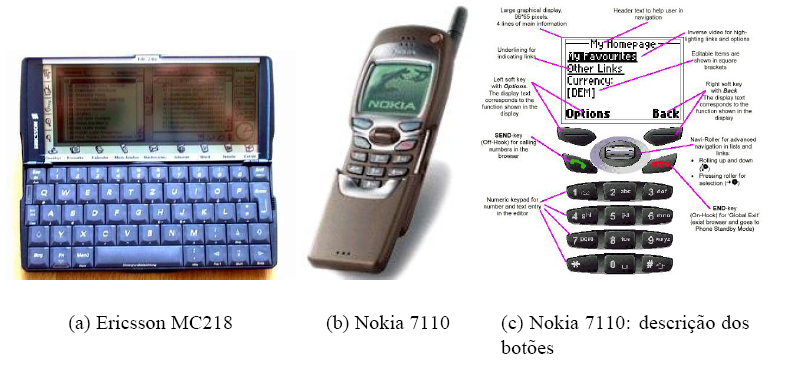
\includegraphics[width=1.00\textwidth]{../Pictures/Baixa/Dispositivos.PNG}
				\label{fig:Dispositivos}
	\end{figure}
\end{frame}

\subsection{Recursos de Hardware}
\begin{frame}
  \frametitle{Desafios e Requisitos no Desenvolvimento e Uso}
  \framesubtitle{Recursos de Hardware}
				\begin{itemize}
					\item Tela reduzida.
					\item Entrada de dados limitada.
					\item Energia limitada.
				\end{itemize}
\end{frame}

%_______________________________________________________________________

\subsection{Recursos de Software}

\begin{frame}

  \frametitle{Desafios e Requisitos no Desenvolvimento e Uso}
  \framesubtitle{Recursos de Software}
				\begin{itemize}
					\item Sistemas Operacionais minimalistas.
					\item API�s limitadas.
					\item Pouca documenta��o para desenvolvimento de m�dio a baixo n�vel.					
				\end{itemize}
\end{frame}

%_______________________________________________________________________
\subsection{Interatividade com o usu�rio}
\begin{frame}
	\frametitle{Desafios e Requisitos no Desenvolvimento e Uso}
  \framesubtitle{Interatividade com o usu�rio.}
				\begin{itemize}
						\item Causa consumo de energia.
		  			\item Telas bem sucintas e informativas.
		  			\item Avisos e solicita��es intuitivas.
				\end{itemize}
\end{frame}

%_______________________________________________________________________
\subsection{Conectividade (Intermit�ncia)}
\begin{frame}
	\frametitle{Desafios e Requisitos no Desenvolvimento e Uso}
  \framesubtitle{Conectividade \textit{(Intermit�ncia)}.}
				\begin{itemize}
					\item Mobilidade.
					\item Largura de banda menor.
					\item Maior taxa de bits errados.
					\item Pagamento pelos servi�os.
				\end{itemize}
\end{frame}